% !TEX encoding = UTF-8
% !TEX TS-program = pdflatex
% !TEX root = ../tesi.tex
% !TEX spellcheck = it-IT

%**************************************************************
\chapter{Project Development}
\label{cap:project-development}
%**************************************************************

\intro{Brevissima introduzione al capitolo}\\

%**************************************************************
\section{SAM file creation}
At first time, to procede with the project, I've created the SAM file by using the \emph{Burrows-Wheeler Aligner} supplied by BWA.

The first command necessary for the file creation is:
\\
\\
\verb|bwa index ref.fa|
\\
\\
This command needs to index the fasta genome file, and that allows the performance increase during the genome alignment.\\

The second typed command is:
\\
\\
\verb|bwa mem ref.fa read1.fq read2.fq > aln-pe.sam|
\\
\\
This command allows the alignment of the two reads file to the genome reference file into a SAM file that needs for the project.\\

There are others different instruments that made this, but BWA should be the best tools specially for the performance.\\

The goal file is a file that contains all the informations about the resequenced genome in according with the SAM specifications.
It weigth about 890MB.


\section{Insertion length}
For this point I wrote an algorithm that for each row of the SAM file that contains informations about the resequencing, I extracted the obtained value from :
\\
\\
\verb|abs(POS -PNEXT)|
\\
\\
Where \emph{POS} is the start of the read and \emph{PNEXT} is the position of the next read.\\
For this point there are some different opinion and come sources, suggests to use only the \emph{TLEN} field of the SAM file.
\\\\
Once time that I extracted all the insertion length, I plotted all the data in a BatChart trak, as yuou could see here \ref{fig:1}, that allows to identify the wrong lectures and the wrong reads.
\\\\
For this trak, a R script was made; from this chart is possible to analize the reads that has wrong insert values, which in some case, are over 2 milion bases long.\\

This error could be explained by the multiple alignment of the genome that align in really far positions.

 \begin{figure}[H]
				\centering
				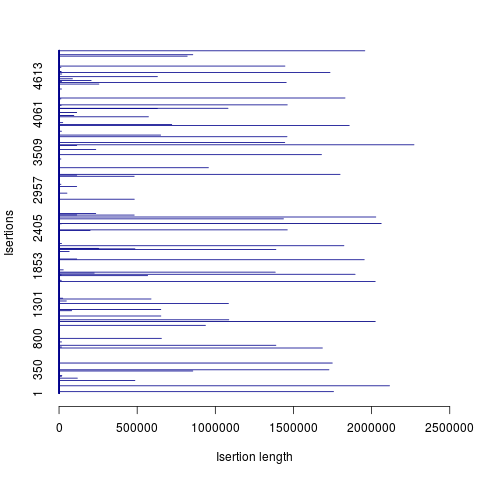
\includegraphics[scale=0.8]{immagini/r.png}
				\caption{Barchart for the isize without exluding errors, the chart include only the first 10.000 reads}\label{fig:1}
				\end{figure}

From this trak, is possibile to see how some read that has the insert lenght longer then 10.000 bases has an error, so for the mean and the standard deviation, this read was be exluded.
As you can see here \ref{fig:2} exludig read with insert longher then 10.000 bases the obtained chart is more right
 \begin{figure}[H]
				\centering
				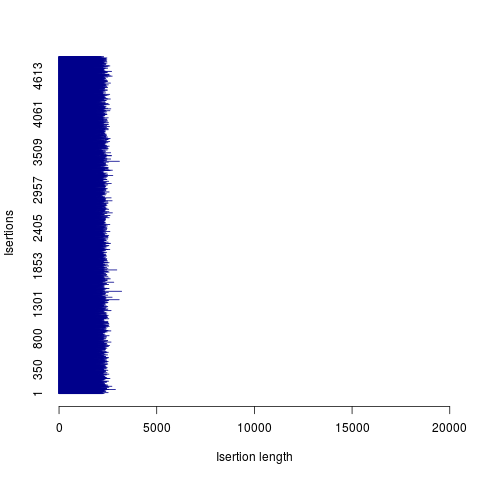
\includegraphics[scale=0.8]{immagini/r1.png}
				\caption{Barchart for the isize with exluding errors}\label{fig:2}
				\end{figure}

The result of mean and standard deviation are:
\begin{itemize}
\item \begin{description}
		\item[MEAN:] 2102
  \end{description}
\end{itemize}

\begin{itemize}
\item \begin{description}
		\item[STD:] 236.84
  \end{description}
\end{itemize}


The result of this point, also, is a csv file that allows to create a barchart with the insertions size with the R script.

\section{Physical Coverage}

The Physical Coverage is calulated by an algorithm really similer to the given perl script.\\

The mainly reason was be the optimization of the algorithm.\\\\

The algorithm, infact, loops on half of reads by checking in the \emph{TLEN} is greather then 0.\\
At first time, I had created an array where each cell was be intialized to 0. 
In each one of these cells, I can put +1 when the index is equal to the read start position, and I can put -1 when the index is equal to the next read start position.\\

Is necessary mentioning who the use read is only the right aligned read, and this filter is made by checking the \emph{FLAG} field of the SAM file.
\\
The resultant values were putted inside a wig file, called \emph{physical\_coverage.wig}.

After that the file was loaded onto IGV to show the physical coverage fort starting to make hypotesys and analisys about some structural variations.

Some small part of resultant trak produced by the IGV are reported below:

 \begin{figure}[H]
				\centering
				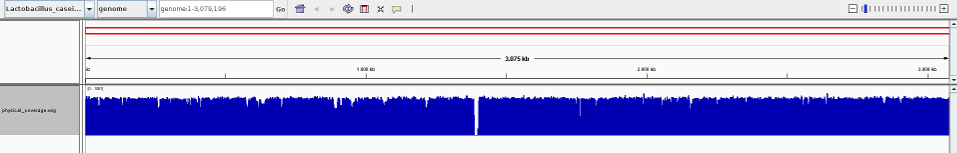
\includegraphics[scale=0.6]{immagini/physical_coverage_1.png}
				\caption{Whole sequence coverage}\label{fig:6}
				\end{figure}


 \begin{figure}[H]
				\centering
				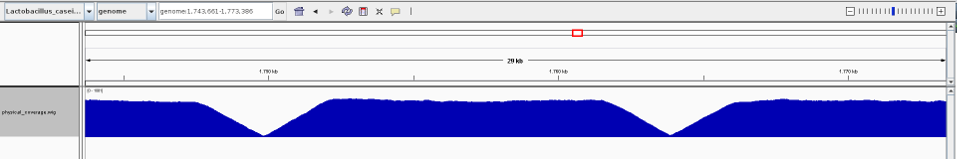
\includegraphics[scale=0.6]{immagini/physical_coverage_2.png}
				\caption{sequence coverage, in the same position the physiscal coerage identify an inversion structural modification}\label{fig:7}
				\end{figure}
				
				
				
 \begin{figure}[H]
				\centering
				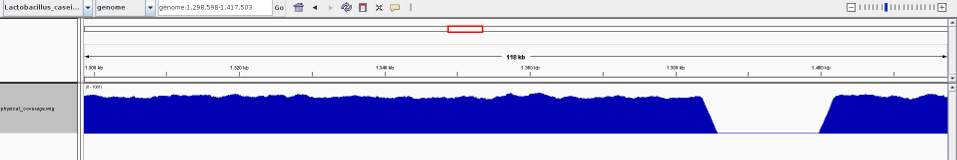
\includegraphics[scale=0.6]{immagini/physical_coverage_3.png}
				\caption{Sequence coverage that identify an structural variation, exactly a long deletation}\label{fig:8}
				\end{figure}				


\section{Sequence Coverage}
The Sequence Coverage is calulated by an algorithm containes inside the SequenceCoverageAlgorithm.py similar to the physical coverage script's but with the differences who is necessary the read that has positive and negative \emph{TLEN}.\\
As well as Physical coverage, also, this algorithm make a check on the \emph{FLAG} fiedl
\\
\\

At first time, I had created an array where each cell was be intialized to 0.
Then for each cell that has with the index between START to START + sequence lenght, I put +1.
This step is necessary for each compatible reads.\\\\

The resultant values were putted inside a wig file, called \emph{sequeence\_coverage.wig}.

After that the file was loaded onto IGV to show the sequence coverage to help to make hypotesys and analisys about some structural variations.

Some small part of resultant trak produced by the IGV are reported below:


 \begin{figure}[H]
				\centering
				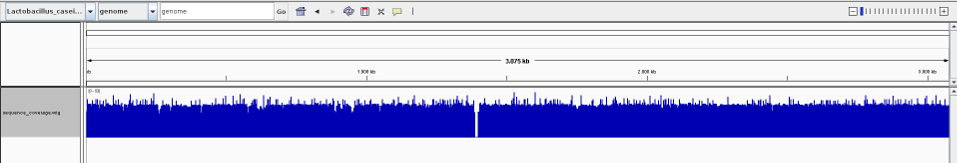
\includegraphics[scale=0.6]{immagini/sequence_coverage_1.png}
				\caption{Whole physical coverage}\label{fig:9}
				\end{figure}


 \begin{figure}[H]
				\centering
				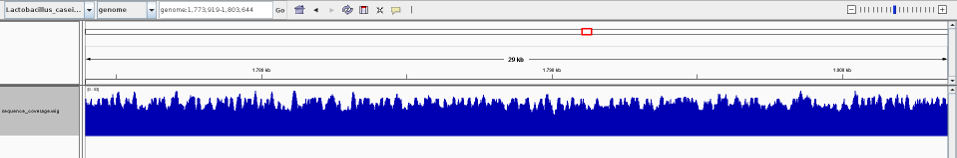
\includegraphics[scale=0.6]{immagini/sequence_coverage_2.png}
				\caption{Physical coverage that identify an structural variation}\label{fig:10}
				\end{figure}
				
				
				
 \begin{figure}[H]
				\centering
				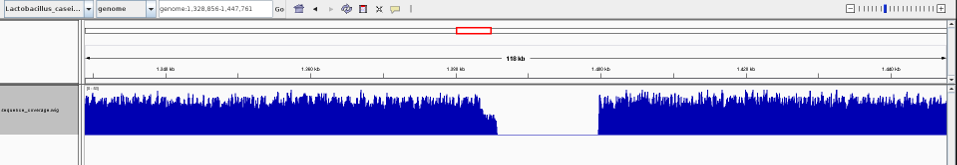
\includegraphics[scale=0.6]{immagini/sequence_coverage_3.png}
				\caption{Physical coverage that identify an structural variation}\label{fig:11}
				\end{figure}	
\section{Kmers counting}
To start talking about the kmers, is necessay to define what is it.
\begin{quote}
The term k-mer typically refers to all the possible substrings of length k that are contained in a string. In computational genomics, k-mers refer to all the possible subsequences (of length k) from a read obtained through DNA Sequencing
\end{quote}

The algorithm for the kmers analisys is inside the KmersAlgorithm.py.\\
to work, the algorithm expects the kmers length value, many different test was made using 7-mers, 4-mers and 9-mers.\\
The result was be really different and to make some hypotesys or analisys was be necessary plot different barchart by usign some R scripts.\\\\

These traks has allowed to learn and see what are the most, and the less present kmers insiede the resequenced genome.\\

The algorithm consider each kmers with the relative opposite, the goal is eliminate the errors that could comes from the "string slicing" from the kmers build.

The algorithm start from position 0 of each \emph{SEQ} and terminate with the end of \emph{SEQ}.
In each loop made on the SEQ string, the algorithm move the start position from \verb|i| to \verb|i+1| and the end position from \verb|end| to \verb|end+1|, the resultant substring is long exactly how we aspect.

I reported the traks generated by the different k dimensions below:

 \begin{figure}[H]
				\centering
				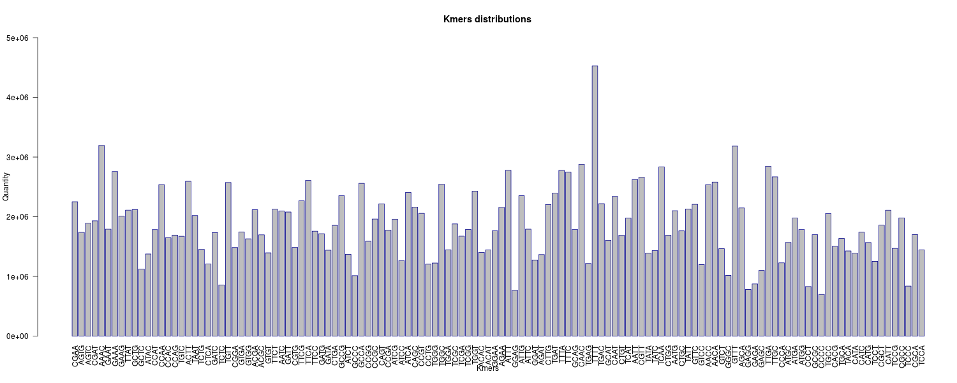
\includegraphics[scale=0.45]{immagini/kmers_4.png}
				\caption{Kmers with k = 4}\label{fig:12}
				\end{figure}


 \begin{figure}[H]
				\centering
				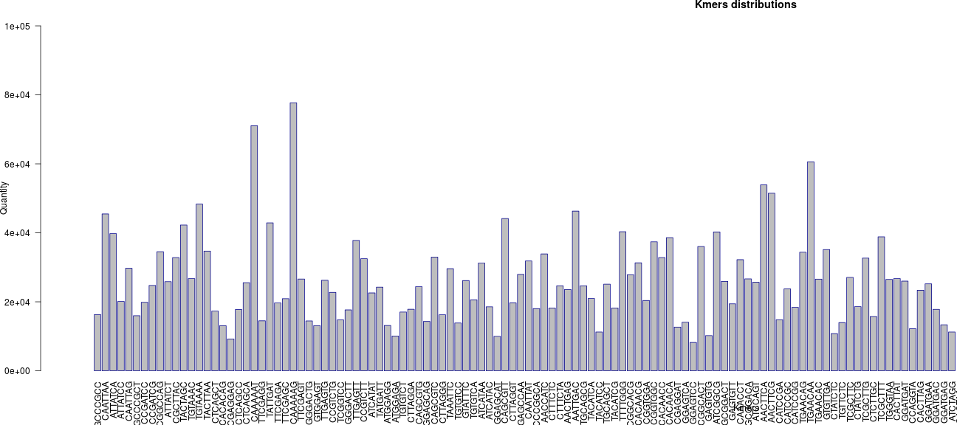
\includegraphics[scale=0.45]{immagini/kmers_7.png}
				\caption{Kmers with k = 7}\label{fig:13}
				\end{figure}
				
				
				
 \begin{figure}[H]
				\centering
				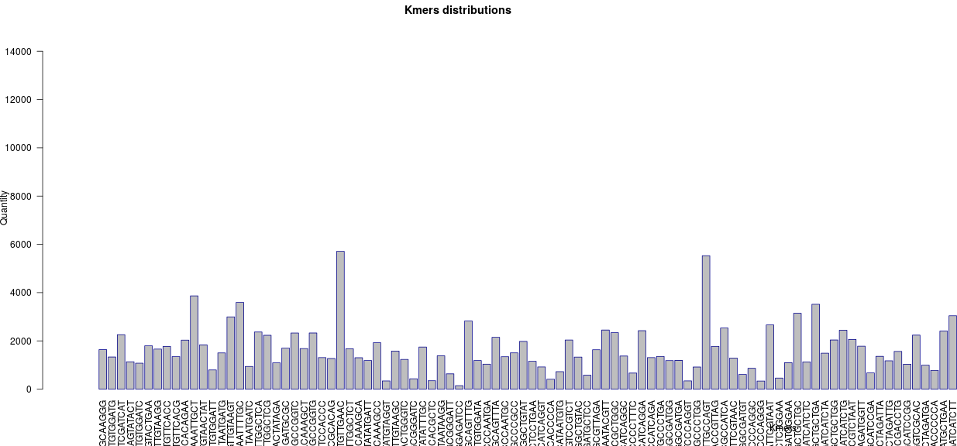
\includegraphics[scale=0.45]{immagini/kmers_9.png}
				\caption{Kmers with k = 9}\label{fig:14}
				\end{figure}	

\section{Cigar H and S reads}